\labeledsection{Introduction to Machine Learning}{sec:ml_intro}
\titledbox{Motivation}{
\begin{itemize}
    \item You have data, and you think there is some \textit{model} that can describe how your data would be generated (if it were)
    \item You do not know that \textit{model}, but you are trying to find something that is as close as possible to that \textit{model} (from some \linkterm{set}{def:set} of \textit{models} (hypotheses) you are willing to consider)
    \item Simplest Example: Learning a \linkterm{function}{function}
    \begin{itemize}
        \item There is a \textbf{target function} $g$ (We do not know it)
        \item We have input-output pairs $X_i = (x, g(x))$ 
        \item The \linkterm{set}{def:set} of hypotheses you are willing to consider are in a space $\mathcal{H}$
        \item Given a \linkterm{set}{def:set} (called training set) of examples $X_i$, we are trying to find a hypothesis $h \in \mathcal{H}$ such that $h \approx g$
    \end{itemize}
\end{itemize}
}

\anondefinition{
A \defemph{Supervised (Inductive) Learning Problem} is the triple $\tuple{\mathcal{H}, T, f}$ where: 
\begin{itemize}
    \item $\mathcal{H}$: The \linkterm{set}{def:set} of \defemph{hypotheses} consisting of \linkterm{functions}{function} $\func{h}{A}{B}$
    \item $T \subseteq \cartprod{A,B}$: A \linkterm{set}{def:set} of \defemph{examples} called the \defemph{Training Set}, such that for every $a \in A$, there is at most one $b \in B$ with $\tuple{a,b} \in T$
\end{itemize}
We \linkterm{assume}{inference_rules_logic} there is an \textit{unknown} \linkterm{function}{function} $\func{f}{A}{B}$ called the \defemph{Target Function} with $T \subseteq f$
}{supervised_learning}

\anondefinition{
\defemph{Inductive Learning Algorithms} solve \linkterm{supervised learning problems}{supervised_learning} by finding a \linkterm{hypothesis}{supervised_learning} $h \in \mathcal{H}$ such that $h \sim f$ (for some notion of similarity)
}{inductive_learning_algorithms}

\anondefinition{
We call a \linkterm{supervised learning problems}{supervised_learning} with \linkterm{target function}{supervised_learning} $\func{f}{A}{B}$ a \defemph{classification problem} if $B$ is \linkterm{finite}{set_cardinality}, and call the \linkterm{members}{def:set} of $B$ \defemph{classes/classifications}. We call it a \defemph{regression problem} if $B = \mathbb{R}$
}{classifcation_regression}


\anondefinition{
We call a \linkterm{hypothesis}{supervised_learning} $h \in \mathcal{H}$ \defemph{consistent with} the unknown target \linkterm{function}{function} $f$ (on a \linkterm{set}{def:set} $T \subseteq \text{dom}(f)$), if it agrees with $f$ (on all \linkterm{examples}{supervised_learning} in $T$)
}{consistent_hyp}

\Example{
Assume we have the following data:
\begin{figure}[H]
    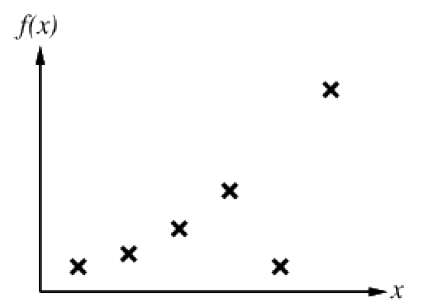
\includegraphics[width=0.25\linewidth]{images/curve_fitting_data.png}
\end{figure}
We can choose our \linkterm{hypotheses space}{supervised_learning} $\mathcal{H}$ to be the linear \linkterm{functions}{function}, then the best linear \linkterm{hypothesis}{supervised_learning} we can find might look like:
\begin{figure}[H]
    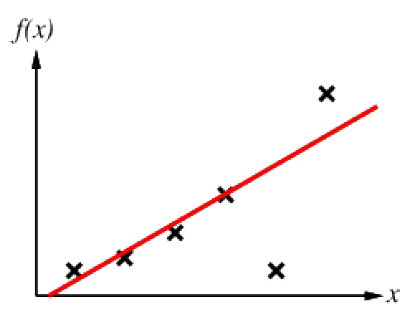
\includegraphics[width=0.25\linewidth]{images/curve_fitting_linear.png}
\end{figure}
Which is \textit{partially, approximately} \linkterm{consistent}{consistent_hyp}.

If $\mathcal{H}$ were the quadratic \linkterm{functions}{function}, we can find another \textit{partially} \linkterm{consistent}{consistent_hyp} \linkterm{hypothesis}{supervised_learning} that might look like:
\begin{figure}[H]
    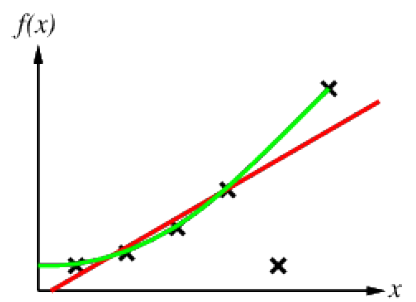
\includegraphics[width=0.25\linewidth]{images/curve_fitting_quadratic.png}
\end{figure}

If we consider Degree$-4$ polynomials, we get a \linkterm{consistent}{consistent_hyp} \linkterm{hypothesis}{supervised_learning}:
\begin{figure}[H]
    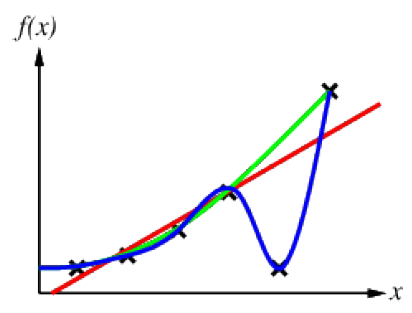
\includegraphics[width=0.25\linewidth]{images/curve_fitting_pold4.png}
\end{figure}

If we consider High-degree polynomials we get more (noisy) \linkterm{consistent}{consistent_hyp} \linkterm{hypotheses}{supervised_learning}, e.g. 
\begin{figure}[H]
    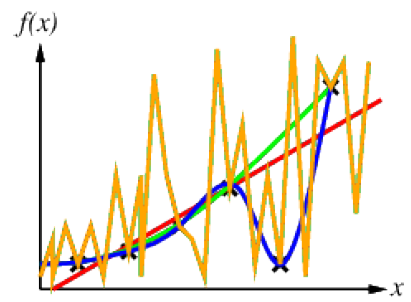
\includegraphics[width=0.25\linewidth]{images/curve_fitting_polhigh.png}
\end{figure}
}{}

\observationbox{
Whether we can find a \linkterm{consistent}{consistent_hyp} \linkterm{hypothesis}{supervised_learning} for a given \linkterm{training set}{supervised_learning} depends on the chosen \linkterm{hypotheses space}{supervised_learning}
}

\titledbox{Recall}{
\textbf{Ockham's-razor:} Maximize a combination of \linkterm{consistency}{consistent_hyp} and simplicity.
}

\anondefinition{
We say that a \linkterm{supervised learning problem}{supervised_learning} is \defemph{realizable}, iff there is a \linkterm{hypothesis}{supervised_learning} $h \in  \mathcal{H}$ that is \linkterm{consistent}{consistent_hyp} on the \linkterm{training set}{supervised_learning} $T$
}{realizable_supervised}

\titledbox{Problem}{
We do not always know whether a given learning problem is \linkterm{realizable}{realizable_supervised}, unless we have prior knowledge. A naive solution would be to make $\mathcal{H}$ as large as possible, e.g. all Turing Machines. However, the complexity of the \linkterm{supervised learning problem}{supervised_learning} is tied to the size of the \linkterm{hypotheses space}{supervised_learning} and \linkterm{consistency}{consistent_hyp} is not even decidable for general Turing Machines.
}

\redbox{
Much of the research in machine learning has concentrated on simple \linkterm{hypotheses spaces}{supervised_learning}
}

\titledbox{Consistency vs. Simplicity}{
Following \textbf{Ockham's Razor}, among competing \linkterm{hypotheses}{supervised_learning}, we prefer those that achieve a good balance between:
\begin{itemize}
    \item \textbf{\linkterm{Consistency}{consistent_hyp}} with the observed \linkterm{training set}{supervised_learning}
    \item \textbf{Simplicity} of the chosen \linkterm{hypothesis}{supervised_learning}
\end{itemize}

This tradeoff is fundamental in machine learning:
\begin{itemize}
    \item If the \linkterm{hypothesis}{supervised_learning} is \textit{too simple}, it may fail to capture important regularities in the data.
    \item If the \linkterm{hypothesis}{supervised_learning} is \textit{too complex}, it may adapt excessively to noise or accidental patterns in the \linkterm{training set}{supervised_learning}.
\end{itemize}
}

\anondefinition{
We say that a \linkterm{hypothesis}{supervised_learning} \defemph{underfits} the data if it is too simple to adequately represent the underlying regularities of the unknown \linkterm{target function}{supervised_learning}. Such \linkterm{hypotheses}{supervised_learning} usually fail to achieve good \linkterm{consistency}{consistent_hyp} even on the \linkterm{training set}{supervised_learning}
}{underfitting}

\anondefinition{
We say that a \linkterm{hypothesis}{supervised_learning} \defemph{overfits} the data if it becomes excessively adapted to the specific \linkterm{training set}{supervised_learning}, including noise or accidental irregularities. Such \linkterm{hypotheses}{supervised_learning} may achieve very high \linkterm{consistency}{consistent_hyp} on the \linkterm{training data}{supervised_learning} while generalizing poorly to unseen \linkterm{examples}{supervised_learning}
}{overfitting}

\titledbox{Bias vs. Variance}{
The tradeoff between simplicity and \linkterm{consistency}{consistent_hyp} is often called the \defemph{Bias-Variance Tradeoff}:
\begin{itemize}
    \item \textbf{High Bias} corresponds to overly simple models that tend to \linkterm{underfit}{underfitting}
    \item \textbf{High Variance} corresponds to overly complex models that tend to \linkterm{overfit}{overfitting}
\end{itemize}
}

\begin{figure}[H]
    \centering
    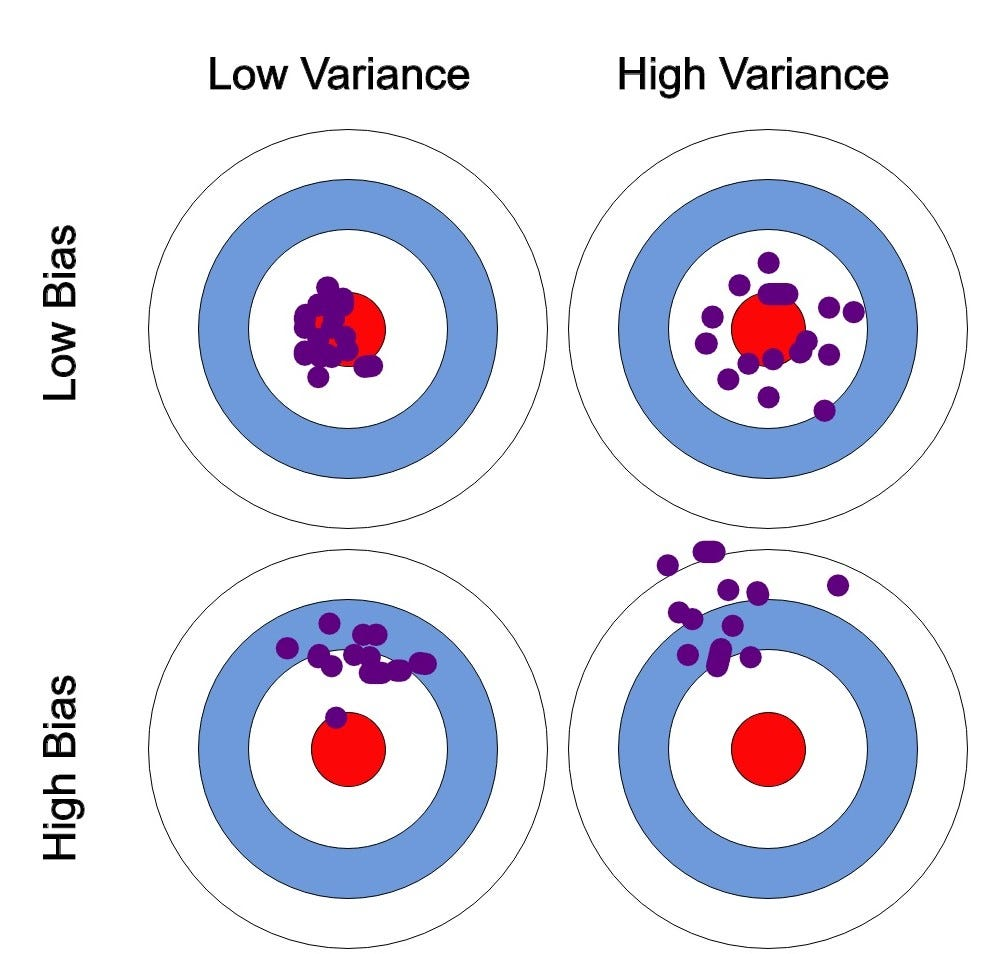
\includegraphics[width=0.4\linewidth]{images/bias_variance.png}
\end{figure}

\titledbox{Why is it called Variance?}{
Imagine repeatedly drawing different random \linkterm{training sets}{supervised_learning} from the same underlying process.

For each \linkterm{training set}{supervised_learning}, we compute the ``best'' \linkterm{hypothesis}{supervised_learning} $h \in \mathcal{H}$.

This generates a sequence of learned \linkterm{hypotheses}{supervised_learning}:
\[
h_1, h_2, h_3, \dots
\]

If small changes in the \linkterm{training set}{supervised_learning} produce large changes in the resulting \linkterm{hypothesis}{supervised_learning}, then the learning method has \defemph{high variance}.

Thus, high variance means the learned model is highly sensitive to the particular sampled data. This sensitivity often causes \linkterm{overfitting}{overfitting}, since the model begins adapting to noise and accidental fluctuations in the training data rather than the underlying structure.
}

\titledbox{Why is it called Bias?}{
Bias measures the systematic error introduced by restricting ourselves to an overly simple \linkterm{hypotheses space}{supervised_learning}.

If the considered \linkterm{hypotheses}{supervised_learning} are all ``far'' from the unknown \linkterm{target function}{supervised_learning}, then even the best possible learned model will make systematic errors.

In this case, the learning method has \defemph{high bias}.

High bias typically causes \linkterm{underfitting}{underfitting}, because the model is too simple to capture important regularities in the data.
}

\observationbox{
In practice, good machine learning models attempt to balance:
\[
\text{simplicity} \quad \text{and} \quad \linkterm{consistency}{consistent_hyp}
\]
or equivalently:
\[
\text{bias} \quad \text{and} \quad \text{variance}
\]

Too much simplicity leads to \linkterm{underfitting}{underfitting}, while too much complexity leads to \linkterm{overfitting}{overfitting}.
}





\problembox{
We want to learn a \linkterm{hypothesis}{supervised_learning} that will best predict future data.
}

\commandnote{
This only works if the \linkterm{training set}{supervised_learning} is \textit{"representative"} of the underlying process.
}

\ideabox{
We think of \linkterm{examples}{supervised_learning} (seen and unseen) as a \linkterm{sequence}{sequence}, and formalize \textit{"representativeness"} via a \textit{stationary assumption} on the \linkterm{probability distribution}{def:prob_distribution}.
}

\redbox{
Each \linkterm{example}{supervised_learning}, before observation, is a \linkterm{random variable}{def:random_variable} $E_j$. The observed value $e_j = \tuple{x_j, y_j}$ is a \linkterm{sample}{def:sample_space} from its \linkterm{distribution}{def:prob_distribution}.
}


\definition{IID}{
A \linkterm{sequence}{sequence} $E_1,E_2,\dots,E_n$ of \linkterm{random variables}{def:random_variable} is \defemph{independent and identically distributed (IID)} iff they are:
\begin{itemize}
  \item \linkterm{independent}{def:independence}, i.e. $\probd{E_j \mid E_{j-1},E_{j-2},\dots}=\probd{E_j}$ for every $j$, and
  \item \defemph{identically distributed}, i.e. $\probd{E_i}=\probd{E_j}$ for every pair of indices $i,j$.
\end{itemize}
}{def:iid}

\definition{Stationary Assumption}{
We assume the sequence $\varepsilon=(E_t)$ of \linkterm{examples}{supervised_learning} is \defemph{stationary} iff for every $k\ge 0$ and every pair of indices $i,j$:
\[
\probd{E_i,\,E_{i+1},\dots,\,E_{i+k}}
=
\probd{E_j,\,E_{j+1},\dots,\,E_{j+k}}.
\]
}{stationarity_assumption_ml}

\commandnote{
\linkterm{Stationarity}{stationarity_assumption_ml} does not imply \linkterm{independence}{def:independence}; \linkterm{IID}{def:iid} implies \linkterm{stationarity}{stationarity_assumption_ml}.
}

\anondefinition{
In \defemph{attribute-based representations}, \linkterm{examples}{supervised_learning} are described by 
\begin{itemize}
    \item \defemph{attributes}: \linkterm{functions}{function} on input samples,
    \item their \defemph{values}, and 
    \item \linkterm{classifcations}{classifcation_regression}
\end{itemize}
}{attribute_based_representations}

\Example{ 
Situations where I will/won't wait for a table in a Restaurant  
\begin{table}[H]
\centering
\caption{The Restaurant Dataset (Russell \& Norvig)}
\label{tab:restaurant_dataset}
\begin{tabular}{c||c|c|c|c|c|c|c|c|c|c||c}
\hline
 & \multicolumn{10}{c||}{\textbf{Attributes}} & \textbf{Target} \\ \cline{2-11}
\textbf{Example} & \textit{Alt} & \textit{Bar} & \textit{Fri} & \textit{Hun} & \textit{Pat} & \textit{Price} & \textit{Rain} & \textit{Res} & \textit{Type} & \textit{Est} & \textit{WillWait} \\ \hline\hline
$X_1$  & T & F & F & T & Some & \$\$\$ & F & T & French  & 0--10  & T \\ 
$X_2$  & T & F & F & T & Full & \$    & F & F & Thai    & 30--60 & F \\ 
$X_3$  & F & T & F & F & Some & \$    & F & F & Burger  & 0--10  & T \\ 
$X_4$  & T & F & T & T & Full & \$    & F & F & Thai    & 10--30 & T \\ 
$X_5$  & T & F & T & F & Full & \$\$\$ & F & T & French  & $>$60  & F \\ 
$X_6$  & F & T & F & T & Some & \$\$   & T & T & Italian & 0--10  & T \\ 
$X_7$  & F & T & F & F & None & \$    & T & F & Burger  & 0--10  & F \\ 
$X_8$  & F & F & F & T & Some & \$\$   & T & T & Thai    & 0--10  & T \\ 
$X_9$  & F & T & F & T & Full & \$    & T & F & Burger  & $>$60  & F \\ 
$X_{10}$ & T & T & T & T & Full & \$\$\$ & F & T & Italian & 10--30 & F \\ 
$X_{11}$ & F & F & F & F & None & \$    & F & F & Thai    & 0--10  & F \\ 
$X_{12}$ & T & T & T & T & Full & \$    & F & F & Burger  & 30--60 & T \\ \hline
\end{tabular}
\end{table}

The \linkterm{attributes}{attribute_based_representations} are:
\begin{itemize}
    \item \textbf{Alt:} Whether a suitable alternative restaurant is available nearby.
    \item \textbf{Bar:} Whether the restaurant has a comfortable bar area to wait in.
    \item \textbf{Fri:} True if the current day is Friday or Saturday.
    \item \textbf{Hun:} Whether the customer is genuinely hungry.
    \item \textbf{Pat:} The number of patrons currently in the restaurant (\textit{None}, \textit{Some}, or \textit{Full}).
    \item \textbf{Price:} The restaurant's price tier (\$, \$\$, or \$\$\$).
    \item \textbf{Rain:} Whether it is actively raining outside.
    \item \textbf{Res:} Whether the customer made a reservation in advance.
    \item \textbf{Type:} The culinary style of the restaurant (\textit{French}, \textit{Thai}, \textit{Burger}, or \textit{Italian}).
    \item \textbf{Est:} The estimated waiting time in minutes (\textit{0--10}, \textit{10--30}, \textit{30--60}, or \textit{$>$60}).
\end{itemize}
}{restaurant_example}

\anondefinition{
For a Boolean \linkterm{classifcation}{classifcation_regression}, we say that an \linkterm{examples}{supervised_learning} is \defemph{positive} ($T$) or \defemph{negative} ($F$) depending on its \linkterm{class}{classifcation_regression}
}{boolean_classification}

\definition{Decision Trees}{
A \defemph{Decision Tree (DT)} for a given \linkterm{attribute-based representation}{attribute_based_representations} is a \linkterm{tree}{tree}, where the \linkterm{non-leaf nodes}{tree} are \linkterm{labeled}{labeled_graph} by \linkterm{attributes}{attribute_based_representations}, their \linkterm{outgoing}{outdegree} \linkterm{edges}{directed_graph} by \linkterm{disjoint}{disjoint} \linkterm{sets}{def:set} of \linkterm{attribute values}{attribute_based_representations}, and the \linkterm{leaf nodes}{tree} are \linkterm{labeled}{labeled_graph} by the \linkterm{classifcations}{classifcation_regression}.
}{decision_trees}

\redbox{\linkterm{Decision Trees}{decision_trees} are one possible representation for \linkterm{hypotheses}{supervised_learning}}

\Example{
Here is the \textit{true} \linkterm{DT}{decision_trees} for \exampleref{restaurant_example}:
\begin{figure}[H]
\centering
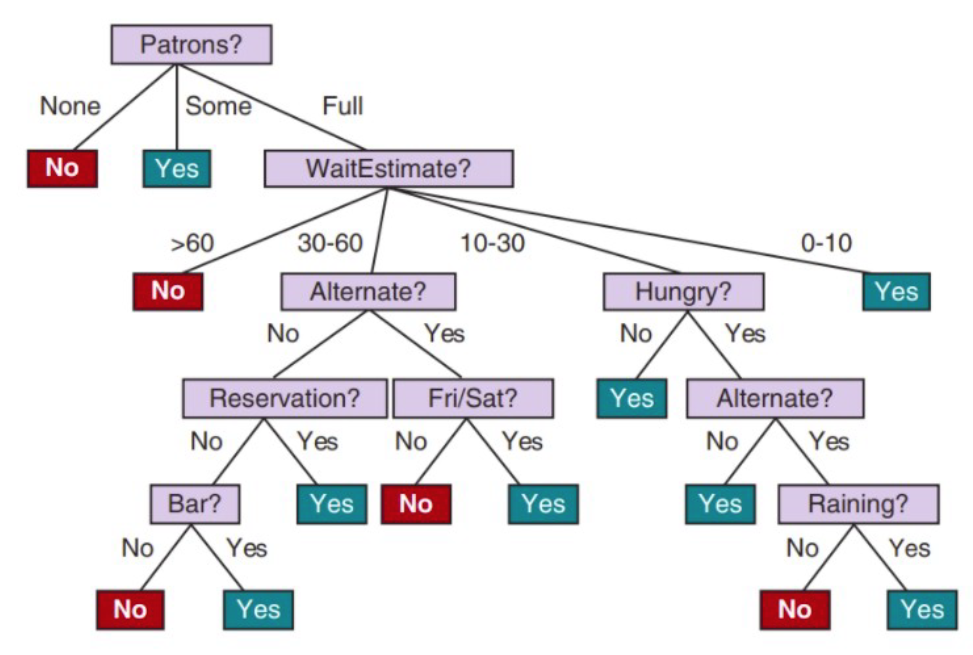
\includegraphics[width=0.4\linewidth]{images/restaurant_true_dt.png}
\caption{The true decision tree for the restaurant dataset.}
\label{fig:restaurant_decision_tree}
\end{figure}
}{}

\anondefinition{
We call an \linkterm{attribute}{attribute_based_representations} together with a \linkterm{set}{def:set} of \linkterm{attribute values}{attribute_based_representations} (an inner node with outgoing edge labels) an \defemph{attribute test}. 
}{attribute_test_dt}

\commandnote{
The \linkterm{target function}{supervised_learning} is a \linkterm{function}{function} $\cartprod{A_1, \cdots, A_n} \to C$, where $A_i$ are the domains of the \linkterm{attributes}{attribute_based_representations}vand $C$ is the \linkterm{set}{def:set} of \linkterm{classifcations}{classifcation_regression}.
}

\redbox{
\linkterm{Decision Trees}{decision_trees} can express any \linkterm{function}{function} of the input \linkterm{attributes}{attribute_based_representations} $\leadsto \mathcal{H} = \cartprod{A_1, \cdots, A_n}$
}

\Example{
For Boolean \linkterm{functions}{function}, a \linkterm{path}{path_graph} from the \linkterm{root}{tree} to a \linkterm{leaf}{tree} corresponds to a row in a truth table (and the \linkterm{DT}{decision_trees} corresponds to a truth table):
\begin{figure}[H]
    \centering
    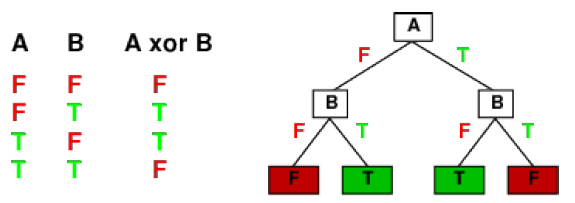
\includegraphics[width = 0.5\linewidth]{images/boolean_dt.png}
\end{figure}
}{}

\problembox{
Trivially, for any \linkterm{training set}{supervised_learning} there is a \linkterm{consistent}{consistent_hyp} \linkterm{hypothesis}{supervised_learning} with one \linkterm{path}{path_graph} to a \linkterm{leaf}{tree} for each \linkterm{example}{supervised_learning}, but it probably won't generalize to new \linkterm{examples}{supervised_learning}. 
}

\solutionbox{
We should find more \textit{compact} \linkterm{Decision Trees}{decision_trees}.
}

\ideabox{
A \textit{good} \linkterm{attribute}{attribute_based_representations} splits the \linkterm{examples}{supervised_learning} into \linkterm{subsets}{subset} that are \textit{ideally} all positive or all negative.
}


